\documentclass{book}
\setlength{\parindent}{0cm}
\usepackage[textwidth=17cm,tmargin=3cm,bmargin=2cm]{geometry}

\usepackage[utf8]{inputenc}
\usepackage[french]{babel}
\usepackage{amsmath,amssymb,amsfonts}

\usepackage{graphicx}
\usepackage{psfrag}
\usepackage{caption}
\usepackage{subcaption}
\usepackage{verbatim}

\usepackage{csquotes}
\usepackage{float}

\usepackage{minted}		% Coloration syntaxique
\usepackage[T1]{fontenc}	% Style de ~ incorrect
\usepackage{lmodern}		% Style de ~ incorrect
%\usemintedstyle{upsud}
\newcommand{\inline}[1]{\mintinline[breaklines]{c++}{#1}}

% Meilleures couleurs
\usepackage{xcolor}
\definecolor{red}{RGB}{221,42,43}
\definecolor{green}{RGB}{132,184,24}
\definecolor{blue}{RGB}{0,72,112}
\definecolor{orange}{RGB}{192,128,64}
\definecolor{gray}{RGB}{107,108,110}

\usepackage[onehalfspacing]{setspace}
\setstretch{1.02}

% Solutions encadrées
\usepackage{tikz}
\usepackage[framemethod=tikz]{mdframed}
\newmdenv[
  singleextra={
    \fill[blue] (P) rectangle ([xshift=-15pt]P|-O);
    \node[overlay,anchor=south east,rotate=90,font=\color{white}] at (P) {\sf\textbf{Correction}};
  },
  firstextra={
    \fill[blue] (P) rectangle ([xshift=-15pt]P|-O);
    \node[overlay,anchor=south east,rotate=90,font=\color{white}] at (P) {\sf\textbf{Correction}};
  },
  secondextra={
    \fill[blue] (P) rectangle ([xshift=-15pt]P|-O);
    \node[overlay,anchor=south east,rotate=90,font=\color{white}] at (P) {\sf\textbf{Correction}};
  },
  backgroundcolor=blue!2,
  linecolor=blue,
  skipabove=12pt,
  skipbelow=12pt,
  innertopmargin=0.4em,
  innerbottommargin=0.4em,
  innerrightmargin=2.7em,
  rightmargin=0.7em,
  innerleftmargin=1.7em,
  leftmargin=0.7em,
]{correction}

% Pour cacher/montrer les solutions, décommenter/commenter les 3 lignes ci-dessous
\usepackage{comment}
% \renewenvironment{correction}{}{}
% \excludecomment{correction}

% Fancy chapters
\makeatletter
  \renewcommand{\@chapapp}{TD}
\makeatother

\usepackage{fancyhdr}
\usepackage{fncychap}
  \ChTitleVar{\Huge\bfseries\sffamily\color{blue}}
  \ChNameVar{\raggedleft\fontsize{22}{16}\selectfont\sffamily\color{blue}}
  \ChNumVar{\raggedleft\fontsize{60}{62}\selectfont\sffamily\color{blue}}

% Fancy sections
\usepackage{titlesec}
\titlespacing*{\chapter}{0pt}{-50pt}{40pt}
\titleformat{\section}[block]
  {\Large\bfseries\sffamily\color{blue}}
  {\thesection}
  {1em}
  {}

\newmdenv[nobreak,backgroundcolor=red!20,roundcorner=10pt,linecolor=white]{warning}

\newenvironment{prompt}{\begin{quote}\color{blue!75}\tt\$\,
}{\end{quote}}

\newcommand{\cc}{\mbox{C}}
\newcommand{\cpp}{\mbox{C\vspace{.5em}\protect\raisebox{.2ex}{\footnotesize++~}}}

\def\filename{\texttt}

\usepackage{hyperref}

\begin{document}


\setcounter{chapter}{5}

\chapter{Tutoriel SFML}

Ce tutoriel a pour but de prendre en main une bibliothèque graphique 2D : la SFML.

\section{Introduction}

La SFML est une bibliothèque C++ d'affichage 2D en temps réel, typiquement pour faire des petits jeux vidéos 2D. Mais c'est aussi très utile pour les simulations en physique !\\

Le principe est très simple : on a une fenêtre, une boucle qui s'exécute à chaque frame (par exemple 30 fois par secondes) et qui affiche des lignes, cercles, rectanges, textes... de toutes tailles et couleurs. Ce n'est toutefois pas conçu pour une utilisation scientifique, et il n'y a rien pour plotter des courbes ou des matrices par exemple. Enfin, il n'y a pas de support pour la 3D, il faudra utiliser d'autres bibliothèques pour cela.\\

Exemples de ce qu'on peut faire rapidement avec :

\begin{center}
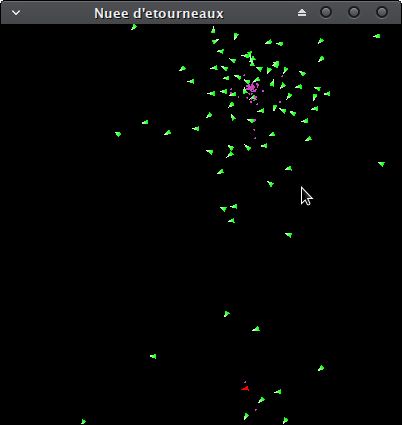
\includegraphics[width=0.48\linewidth]{Tuto_SFML/ex_SFML_1.png}
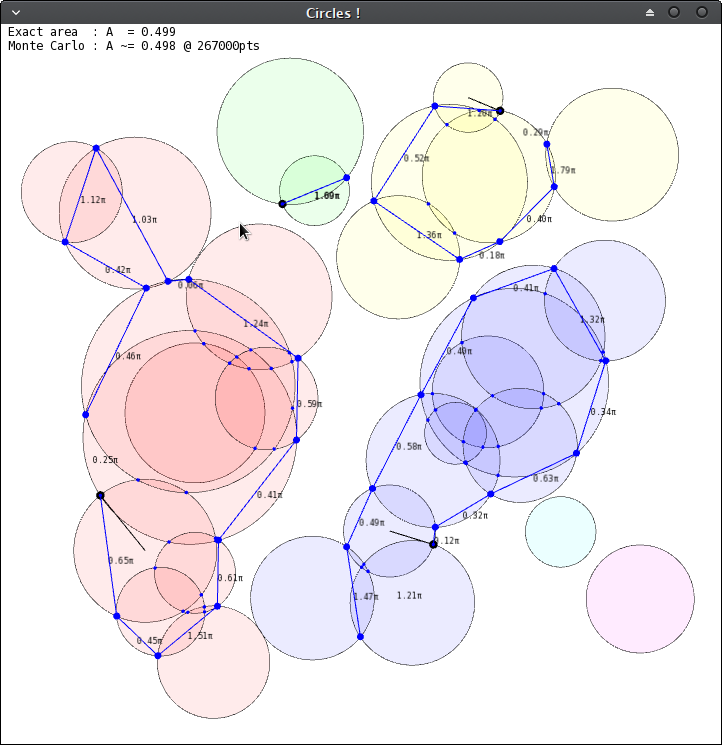
\includegraphics[width=0.49\linewidth]{Tuto_SFML/ex_SFML_2.png}
\end{center}

\section{Installation de la SFML}

Une bibliothèque (\emph{library} en anglais) n'est rien d'autre qu'un ensemble de code cohérent, auto-contenu et disposant d'une interface claire et utilisable même pour quelqu'un qui ne maîtrise pas les rouages internes.\\

En C++, les fonctions et classes sont exposées à travers les fichiers d'en-tête (\emph{headers}, \filename{.h} ou \filename{.hpp}), et l'implémentation est en général compilée sous forme d'un fichier objet. Pour utiliser une bibliothèque, il faut
\begin{itemize}
  \item inclure le ou les fichiers d'en-tête dans le code aux endroits où on utilise la bibliothèque (\texttt{\#include <mylib.h>} par exemple)
  \item ajouter le ou les fichiers objets lors de l'édition de lien (\texttt{g++ ... -lmylib -o ...} par exemple)
\end{itemize}

Pour les langages compilés, dont le \cpp, il existe deux types de fichiers objets :
\begin{itemize}
  \item les bibliothèques \emph{statiques} (fichiers \texttt{.a}), qui ne sont rien d'autre qu'une archive de \texttt{.o} qui sont \emph{copiés} et liés dans l'exécutable comme n'importe quel autre \texttt{.o}; l'exécutable contient alors tout ce qui est nécessaire pour l'exécution, et est facile à distribuer
  \item les bibliothèques \emph{dynamiques}, ou \emph{partagées} (fichiers \texttt{.so} sur Linux, \texttt{.dylib} sur macOS, \texttt{.dll} sur Windows), qui sont des fichiers objets qui ne sont pas copiés dans l'exécutable, et qui doivent donc être livrés avec l'exécutable ou être déjà installés au niveau du système; c'est très souvent le cas de la bibliothèque standard \cpp, qu'il serait inefficace de re-livrer pour chaque programme\footnote{C'est certes plus complexe. Mais il y a un gros avantage des bibliothèques partagées : si $N$ programmes utilisent la même bibliothèque, le système d'exploitation n'a besoin de charger le \texttt{.so} qu'une seule fois en mémoire, ce qui ne serait pas le cas pour une édition de lien statique où, sans le savoir, le même code machine serait chargé $N$ fois en mémoire. Ce joli mécanisme est exploité au maximum sur les systèmes Linux où la bibliothèques sont installées par le gestionnaire de paquet, et non livrées avec l'exécutable; c'est moins le cas sur Windows et macOS. Autre avantage : les bibliothèques peuvent être mises à jour sans avoir à ré-installer le programme. Désavantage : il faut que l'ensemble soit cohérent, ce qui serait pénible sans un gestionnaire de paquets. D'une certaine manière, c'est aussi le cas dans l'écosystème Python, bien que les bibliothèques sont sous forme de code source et non de code machine.}.
\end{itemize}
Le compilateur ira chercher les fichiers d'en-tête et objets (et le chargeur de programme les bibliotèques paratgées) à des endroits prédéfinis et standardisés. Sur Linux et macOS, les fichiers d'en-tête sont en général dans \filename{/usr/include} ou \filename{/usr/local/include}, et les fichiers objets dans \filename{/usr/lib} ou \filename{/usr/local/lib}. Il est toutefois possible de dire au compilateur d'aller chercher ailleurs, comme on le verra.

\vspace{1em}

Pour la plupart des langages de programmation, il y a trois façons d'installer une bibliothèque :
\begin{enumerate}
  \item télécharger le code source, compiler la bibliothèque (si nécessaire), et placer les fichiers résultants au bon endroit (cet endroit varie suivant le langage)
  \item télécharger la bibliothèque déjà compilée (on parle de fichiers binaires) et placer les fichiers au bon endroit
  \item utiliser le gestionnaire de paquets du système ou du langage (lorsqu'il existe et lorsque la bibliothèque a été empaqutée par la communauté) faire ces opérations automatiquement (\texttt{pip install ...} en Python, \texttt{apt install ...} sur les systèmes Linux de la famille Debian/Ubuntu, \texttt{pacman -S ...} sur ArchLinux, \texttt{brew install ...} sur macOS...)
\end{enumerate}

Ceux disposants de leur propre ordinateur préfèreront la dernière option. Sur les machines du $\hbar$, la SFML n'est pas installée et vous ne disposez pas des droits pour installer un paquet via \texttt{apt}. Il faut donc se rabattre sur une des deux premières options. La deuxième option est décrite sur la page \url{https://www.sfml-dev.org/tutorials/2.5/start-linux-fr.php}. La première est décrite dans la section \ref{sec:Compilation et installation dans un dossier local} ci-dessous.

\subsection{Installation sur un Linux de la famille Debian avec droits d'administrateur}

On utilise le gestionnaire de paquets \texttt{apt}. Il suffit de faire \texttt{apt install libsfml-dev} avec droits d'administrateurs. Le postfixe \texttt{dev} est là pour indiquer que l'on souhaite installer les fichiers d'en-tête. On ne peut pas le faire sur les machines du $\hbar$ car on ne dispose pas des droits d'administrateurs.

\subsection{Compilation et installation dans un dossier local}
\label{sec:Compilation et installation dans un dossier local}

Il faut déjà télécharger le code source de la SMFL, qu'on peut trouver sur \url{https://www.sfml-dev.org/download-fr.php}. Choisir "Dernière version stable", puis "Tout OS" et "Code source". Une fois le téléchargement effectuer, on ouvre un terminal et on se place dans le dossier de téléchargement.

Ensuite, on décompresse et on se place dans le dossier :
\begin{minted}{shell-session}
$ unzip SFML-*-sources.zip
$ cd SFML-*
$ ls
\end{minted}

L'auteur de la bibliothèque SMFL a choisi \texttt{cmake} pour la construction de la bibliothèque. C'est un outil très populaire pour générer des \texttt{Makefile} facilement\footnote{Il n'y a pas assez de temps pour introduire cet outil dans le cours, mais n'hésitez pas à l'utiliser pour vos projets !}. La bonne pratique est de créer un dossier \texttt{build} et de se placer dedans pour compiler la bibliothèque. On appelle alors \texttt{cmake} :

\begin{minted}[breaklines]{shell-session}
$ mkdir build && cd build
$ cmake -DSFML_BUILD_AUDIO=False -DBUILD_SHARED_LIBS=True -DCMAKE_INSTALL_PREFIX=$HOME/usr -DSFML_PKGCONFIG_INSTALL_PREFIX=$HOME/usr/lib/pkgconfig ..
\end{minted}
avec les options suivantes :
\begin{itemize}
  \item \mintinline{text}{SFML_BUILD_AUDIO=False} pour désactiver les fonctionnalité audio (il manque des bibliothèques sur le système des machines du $\hbar$ pour les utiliser)
  \item \mintinline{text}{BUILD_SHARED_LIBS=True} pour qu'une bibliothèque \emph{partagée} soit générée
  \item \mintinline{text}{CMAKE_INSTALL_PREFIX=$HOME/usr} et \mintinline{text}{SFML_PKGCONFIG_INSTALL_PREFIX=$HOME/usr/lib/pkgconfig} pour que la bibliothèque soit intallée dans votre dossier utilisateur (\mintinline{shell-session}{$HOME}), sous le préfixe \mintinline{text}{~/usr/}; on ne peut en effet intaller la bibliothèque sous le préfixe standard \mintinline{text}{/usr/} car on n'a pas de droits d'administrateur sur les machines du $\hbar$...
\end{itemize}

\vspace{1em}
Enfin, on compile et on installe les fichiers à l'endroit désiré :

\begin{minted}[breaklines]{shell-session}
$ make
$ make install
\end{minted}

Regardez la sortie de \texttt{make install} et vérifiez que les fichiers ont étés installés au bon endroit. Passez un peu de temps à regarder l'organisation de \mintinline{text}{~/usr/}, ainsi que du répertoire système \mintinline{text}{/usr/}. En particulier, trouvez les fichiers objet de la SFML ainsi que les fichiers d'en-tête. La très grande majorité des bibliothèques sont organisées de cette sorte.

\section{Premiers pas avec la SFML}

On trouvera de bons tutoriels sur le site officiel : \url{https://www.sfml-dev.org/tutorials/2.5/index-fr.php}. Les sections qui nous concernent le plus sont "\href{https://www.sfml-dev.org/tutorials/2.5/window-window-fr.php}{Ouvrir et gérer une fenêtre SFML}", "\href{https://www.sfml-dev.org/tutorials/2.5/graphics-draw-fr.php}{Dessiner avec SFML}", et "\href{https://www.sfml-dev.org/tutorials/2.5/graphics-shape-fr.php}{Dessiner des formes}".\\

\newpage
Voici un exemple de \inline{main()} typique :
\begin{center}
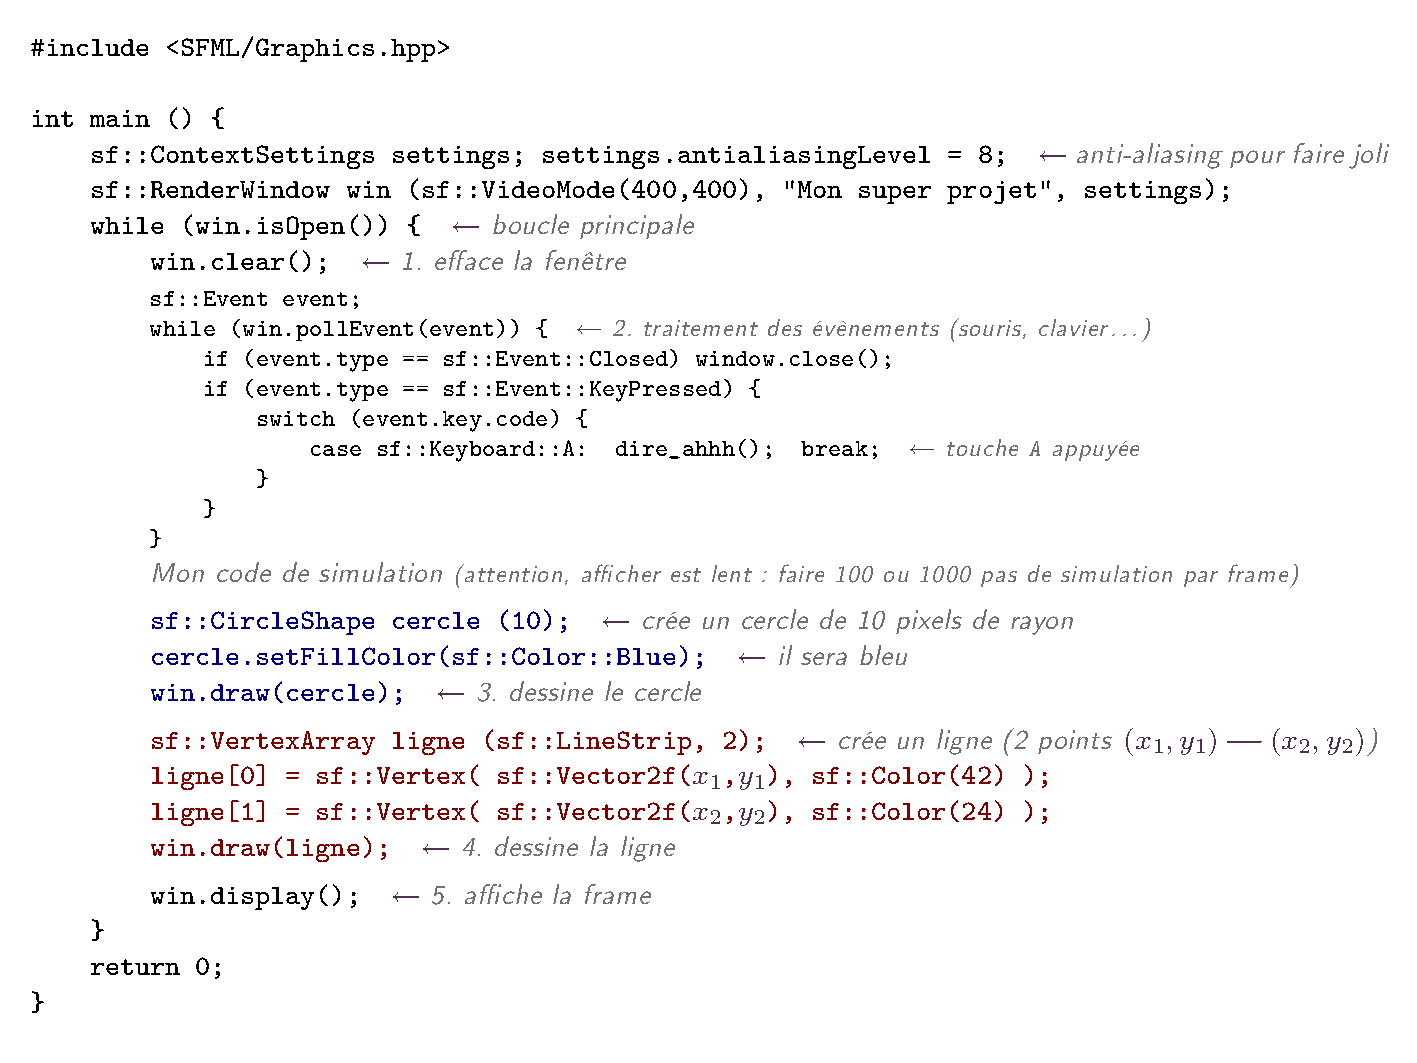
\includegraphics[width=0.95\linewidth]{Tuto_SFML/template_main_sfml.pdf}
\end{center}

Créez un nouveau dossier de travail et créez un fichier \filename{main.cpp} contenant l'exemple de la page "\href{https://www.sfml-dev.org/tutorials/2.5/graphics-draw-fr.php}{Dessiner avec SFML}". À l'emplacement approprié dans le code, ajoutez
\begin{minted}[breaklines,fontsize=\footnotesize]{c++}
// construction d'un rectangle de largeur 120 et hauteur 50
sf::RectangleShape rectangle (sf::Vector2f(120, 50));
// change sa couleur en violet (R=1, G=0, B=1)
rectangle.setFillColor(sf::Color(255,0,255));
// définit sa position (haut gauche) à (x,y)=(150,50)
rectangle.setPosition(150, 50);
// dessin du rectange
window.draw(rectangle);
\end{minted}

Note : Comme bien souvent dans les systèmes d'affichage, les positions $(x,y)$ sont exprimées \emph{en pixels par rapport au coin haut gauche}, contraire à l'usage des physiciens de placer l'origine en bas à gauche. Lorsque l'on augmente $y$, le rectangle descent sur l'écran !\\

Pour compiler ce programme de test, il va falloir dire au compilateur de prendre en compte la bibliothèque.

\subsection{Avec une installation au niveau du système}

C'est très simple. Comme la bibliothèque est installée à un emplacement standard, le compilateur sait déjà où chercher les fichiers d'en-tête et les fichiers objets. Il suffit juste de dire au linker de lier la bibliothèque à l'exécutable :

\begin{minted}[breaklines]{shell-session}
$ g++ -c main.cpp -o main.o  # compilation
$ g++ main.o -lsfml-graphics -lsfml-system -lsfml-window -o test.exe  # édition de liens
$ ./test.exe
\end{minted}

Pour dire au linker de lier un fichier objet de bibliothèque, par exemple \filename{libmachin.so}, on lui passe le flag \texttt{-lmachin}. La SFML est en fait séparée en plusieurs module, et pour un simple affichage graphique, il faut
\begin{itemize}
  \item \texttt{sfml-system} (routines système)
  \item \texttt{sfml-window} (création de fenêtres dans l'interface graphique et contexte OpenGL)
  \item \texttt{sfml-graphics} (routines de dessin)
\end{itemize}

\subsection{Avec une installation dans un dossier local}

Dans ce cas, les fichiers de la bibliothèque ne sont pas dans un répertoire standard, et il faut dire au compilateur et au linker où ils te trouvent avec les flags \texttt{-I} et \texttt{-L}, le tilde \texttt{\raisebox{0.5ex}{\texttildelow}/...} représentant le dossier personnel :

\begin{minted}[breaklines]{shell-session}
$ g++ -I$HOME/usr/include -c main.cpp -o main.o  # compilation
$ g++ main.o -L$HOME/usr/lib -lsfml-graphics -lsfml-system -lsfml-window -o test.exe  # édition de liens
$ ./test.exe
\end{minted}

Essayez l'exécution. Pourquoi, à votre avis, le système d'exploitation refuse d'exécuter \filename{test.exe} ? Pour résoudre le problème, le plus simple est sans doute de rajouter un flag \texttt{rpath} à l'édition de lien :
\begin{minted}[breaklines]{shell-session}
$ g++ -I$HOME/usr/include -c main.cpp -o main.o  # compilation
$ g++ main.o -L$HOME/usr/lib -lsfml-graphics -lsfml-system -lsfml-window -Wl,-rpath,$HOME/usr/lib -o test.exe  # édition de liens
$ ./test.exe
\end{minted}

\subsection{Animation}

Ajoutez une varible globale \inline{float anim;} que vous incrémentez de \inline{0.01} à chaque itération de la boucle d'affichage. Faites osciller la position du rectangle en, par exemple, rajoutant \inline{10 * sin(anim)} à la position $x$.

\begin{correction}
\begin{minted}[fontsize=\footnotesize,mathescape,xrightmargin=0.5cm,xleftmargin=0.5cm]{c++}
#include <SFML/Graphics.hpp>
#include <cmath>
using namespace std;

int main () {
    // création de la fenêtre
    sf::RenderWindow window(sf::VideoMode(800, 600), "Mon super rectangle");

    float anim = 0;

    // on fait tourner le programme en boucle
    while (window.isOpen()) {
        // gestion des évènements (non nécessaire ici)
        // ...

        // effacement de la fenêtre en noir
        window.clear(sf::Color::Black);

        // c'est ici qu'on dessine tout
        // construction d'un rectangle de 120 par 50
        sf::RectangleShape rectangle (sf::Vector2f(120, 50));
        // change sa couleur en rouge (R=255, G=0, B=0)
        rectangle.setFillColor(sf::Color(255,0,255));
        // définit sa position à (x,y)=(150,50)
        rectangle.setPosition(150+20*sin(anim), 50);
        // dessin du rectange
        window.draw(rectangle);

        // affichage de tout ce qu'on a dessiné
        window.display();

        // animation
        anim += 0.01;
    }

    return 0;
}
\end{minted}
\end{correction}

\end{document}
